% Chapter 3, Section 1: Probability Distributions

\section{Probability Distributions \difficultyInline{beginner}}
\label{sec:probability-distributions}

Probability distributions are mathematical functions that describe how probabilities are distributed across different possible outcomes of a random variable, providing the fundamental framework for modeling uncertainty in data and making predictions in machine learning and deep learning applications.

\subsection{Intuition: What is Probability?}

Imagine you're playing a game of dice where you roll a standard six-sided die with numbers 1 through 6. Before rolling, you know that each face has an equal chance of appearing, meaning that if you roll the die many times, each number will appear approximately one-sixth of the time. This "chance" is what we call probability - a number between 0 and 1 that quantifies how likely an event is to occur, where 0 means impossible and 1 means certain. In machine learning, we face uncertainty everywhere, from data uncertainty about whether the next customer will click on an ad, to model uncertainty about how confident our neural network is in its prediction, to parameter uncertainty about what the best value is for our model's weights. Probability distributions are mathematical tools that help us model and work with this uncertainty systematically, providing a rigorous framework for making decisions under uncertainty and quantifying the confidence we can have in our predictions and model parameters.

\subsection{Visualizing Probability}

Consider a simple example: predicting whether it will rain tomorrow. We might say there's a 30\% chance of rain, which means that if we could repeat tomorrow 100 times, rain would occur about 30 times, the probability of rain is 0.3, and the probability of no rain is 0.7. This intuitive understanding of probability helps us visualize how probability distributions work - they assign numerical values to different outcomes, showing us not just what can happen, but how likely each outcome is to occur.

\begin{figure}[h]
\centering
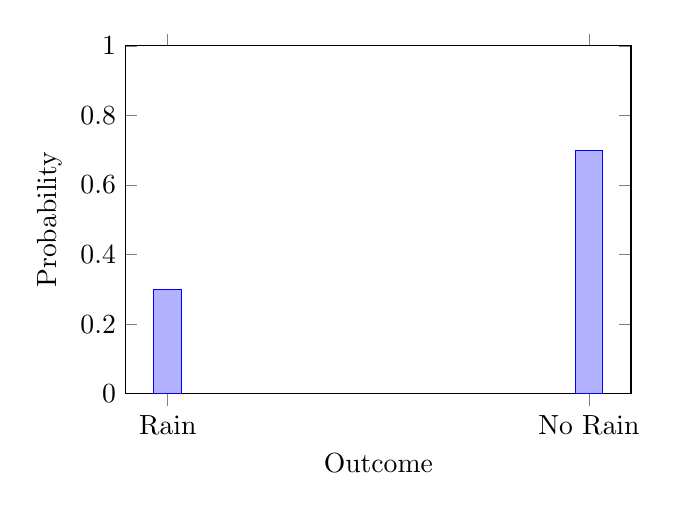
\begin{tikzpicture}
\begin{axis}[
    ybar,
    ylabel={Probability},
    xlabel={Outcome},
    xtick={1,2},
    xticklabels={Rain, No Rain},
    ymin=0,
    ymax=1,
    width=8cm,
    height=6cm
]
\addplot coordinates {(1,0.3) (2,0.7)};
\end{axis}
\end{tikzpicture}
\caption{Probability distribution for rain prediction}
\label{fig:rain-probability}
\end{figure}

Probability theory provides a mathematical framework for quantifying uncertainty. In deep learning, we use probability distributions to model uncertainty in data, model parameters, and predictions.

\subsection{Discrete Probability Distributions}

Discrete probability distributions deal with outcomes that can be counted and listed explicitly, such as coin flips with heads or tails, dice rolls with numbers 1 through 6, or email classification with spam or not spam. These distributions assign probabilities to each possible outcome, where the sum of all probabilities equals 1, representing the fact that one of the possible outcomes must occur.

A discrete random variable $X$ takes values from a countable set. The \textbf{probability mass function} (PMF) $P(X=x)$ assigns probabilities to each possible value:

\begin{equation}
P(X=x) \geq 0 \quad \text{for all } x
\end{equation}

\begin{equation}
\sum_{x} P(X=x) = 1
\end{equation}

\subsubsection{Example: Fair Coin}

For a fair coin, we have:
\begin{align}
P(X=0) &= 0.5 \quad \text{(Tails)} \\
P(X=1) &= 0.5 \quad \text{(Heads)}
\end{align}

\begin{figure}[h]
\centering
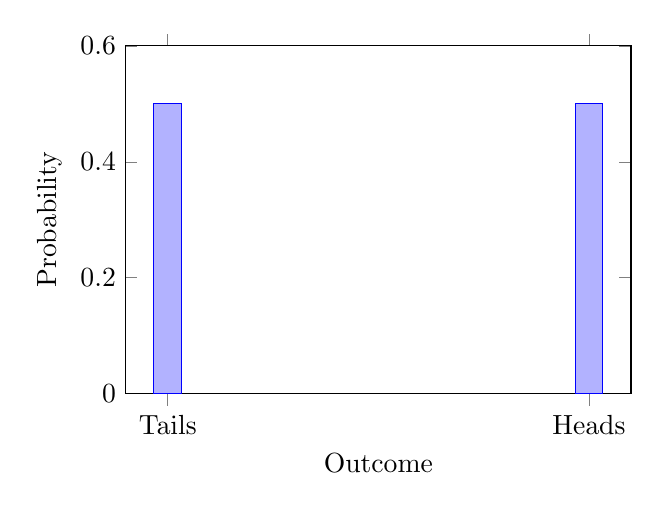
\begin{tikzpicture}
\begin{axis}[
    ybar,
    ylabel={Probability},
    xlabel={Outcome},
    xtick={0,1},
    xticklabels={Tails, Heads},
    ymin=0,
    ymax=0.6,
    width=8cm,
    height=6cm
]
\addplot coordinates {(0,0.5) (1,0.5)};
\end{axis}
\end{tikzpicture}
\caption{Probability mass function for a fair coin}
\label{fig:coin-pmf}
\end{figure}

\subsection{Continuous Probability Distributions}

Continuous probability distributions deal with variables that can take any value within a continuous range, such as the height of people which can be 170 cm, 170.5 cm, 170.52 cm, and so on, or temperature which can be 22.3°C, 22.34°C, 22.341°C, and so on, or neural network weights which can be 0.1234, 0.12345, 0.123456, and so on. Since there are infinitely many possible values, we can't assign probabilities to individual points, but instead use density functions that describe how "concentrated" the probability is in different regions of the continuous space.

A continuous random variable can take any value in a continuous range. We describe it using a \textbf{probability density function} (PDF) $p(x)$:

\begin{equation}
p(x) \geq 0 \quad \text{for all } x
\end{equation}

\begin{equation}
\int_{-\infty}^{\infty} p(x) \, dx = 1
\end{equation}

The probability that $X$ falls in an interval $[a, b]$ is:

\begin{equation}
P(a \leq X \leq b) = \int_a^b p(x) \, dx
\end{equation}

\subsubsection{Example: Normal Distribution}

The most common continuous distribution is the \textbf{normal (Gaussian) distribution}, which looks like a bell curve:

\begin{figure}[h]
\centering
\begin{tikzpicture}
\begin{axis}[
    ylabel={Probability Density},
    xlabel={Value},
    domain=-3:3,
    width=10cm,
    height=6cm,
    samples=100,
    grid=major,
    grid style={line width=.1pt, draw=gray!10},
    major grid style={line width=.2pt, draw=gray!50}
]
\addplot[bookpurple, thick] {1/sqrt(2*pi) * exp(-x^2/2)};
\addplot[bookred, thick] {1/sqrt(2*pi*0.5) * exp(-(x-0.5)^2/(2*0.5))};
\end{axis}
\end{tikzpicture}
\caption{Two normal distributions with different means and standard deviations. The purple curve shows $\mathcal{N}(0, 1)$ (standard normal with mean 0 and variance 1), while the red curve shows $\mathcal{N}(0.5, 0.5)$ (normal with mean 0.5 and variance 0.5). The grid helps visualize the density values at different points.}
\label{fig:normal-distributions}
\end{figure}

The area under the curve between any two points gives the probability of the variable falling in that range.

\begin{figure}[h]
\centering
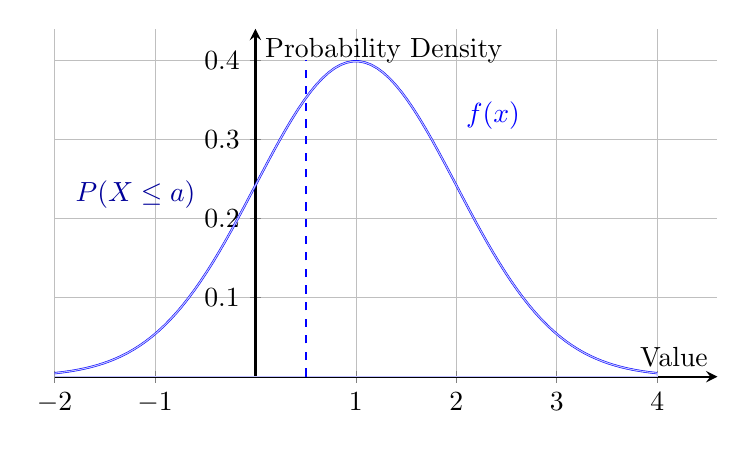
\begin{tikzpicture}
\begin{axis}[
    ylabel={Probability Density},
    xlabel={Value},
    domain=-2:4,
    width=10cm,
    height=6cm,
    samples=100,
    grid=major,
    grid style={line width=.1pt, draw=gray!10},
    major grid style={line width=.2pt, draw=gray!50},
    axis lines=middle,
    axis line style=thick,
    enlargelimits=upper
]
% Normal distribution
\addplot[blue,thick] {1/sqrt(2*pi) * exp(-(x-1)^2/2)};
% Fill area under curve from -2 to 0.5
\addplot[blue!25, fill opacity=0.3] {1/sqrt(2*pi) * exp(-(x-1)^2/2)} \closedcycle;
% Vertical line at a=0.5
\addplot[blue,dashed,thick] coordinates {(0.5,0) (0.5,0.4)};
\node[blue,below] at (axis cs:0.5,0) {$a$};
\node[blue,above right] at (axis cs:2,0.3) {$f(x)$};
\node[blue!60!black,above left] at (axis cs:-0.5,0.2) {$P(X\leq a)$};
\end{axis}
\end{tikzpicture}
\caption{Cumulative probability visualization showing the probability density function $f(x)$ and the cumulative probability $P(X \leq a)$ for a normal distribution. The shaded area represents the probability that the random variable $X$ takes a value less than or equal to $a$.}
\label{fig:cumulative-probability}
\end{figure}

\subsection{Joint and Marginal Distributions}

In real-world scenarios, we often deal with multiple variables simultaneously, such as weather prediction involving both temperature and humidity, image classification involving pixel values at different positions, or stock prices involving multiple stocks in a portfolio. The joint distribution tells us about the probability of combinations of values across all variables, while marginal distributions tell us about individual variables when we ignore the others, providing a way to understand both the relationships between variables and the behavior of individual variables in isolation.

\subsubsection{Example: Weather Data}

Consider a simple weather dataset with two variables:
\begin{itemize}
    \item $X$: Temperature (Hot/Cold)
    \item $Y$: Humidity (High/Low)
\end{itemize}

\begin{table}[h]
\centering
\begin{tabular}{|c|c|c|c|}
\hline
 & $Y=$ High & $Y=$ Low & \textbf{Marginal} \\
\hline
$X=$ Hot & 0.3 & 0.2 & \textbf{0.5} \\
$X=$ Cold & 0.1 & 0.4 & \textbf{0.5} \\
\hline
\textbf{Marginal} & \textbf{0.4} & \textbf{0.6} & \textbf{1.0} \\
\hline
\end{tabular}
\caption{Joint probability table for weather data}
\label{tab:weather-joint}
\end{table}

For multiple random variables $X$ and $Y$, the \textbf{joint distribution} $P(X, Y)$ describes their combined behavior. The \textbf{marginal distribution} is obtained by summing (or integrating) over the other variable:

\begin{equation}
P(X=x) = \sum_{y} P(X=x, Y=y)
\end{equation}

For continuous variables:

\begin{equation}
p(x) = \int p(x, y) \, dy
\end{equation}

From our weather example:
\begin{itemize}
    \item $P(X=\text{Hot}) = 0.3 + 0.2 = 0.5$ (marginal probability of hot weather)
    \item $P(Y=\text{High}) = 0.3 + 0.1 = 0.4$ (marginal probability of high humidity)
\end{itemize}
